% !Mode:: "TeX:UTF-8"
\mychapter{基于二维码的图像识别单向传输系统}
\label{cha:sys}

基于上文的复杂环境下的高效自适应二维码编解码,现在我们有能力在屏幕-摄像机的物理信道上构建真正的逻辑传输信道,从而实现本项目要求的单项文件传输隔离系统。本章主要着重于软件层面,介绍在物理设备上构建单向传输系统的实现过程及其细节。

\section{软件整体架构}

本项目采用Rust,C与C++语言开发,二维码的编码采用Rust的QRCode-Rust, 解码采用Bar-Decoder,均基于本项目的使用场景做了特异性优化与改进;多线程采用RUST原生线程实现构建线程池;进程间通信采用ZeroMQ。系统运行于Ubuntu 20.04系统中,Rust使用采用Version 2018。

\subsection{流程架构}

图像识别单向隔离装置技术架构从下到上分为五层,分别为:物理层、编解码层、数据封装层、数据链路层和网络接口层,包括服务和协议有:二维码编码服务、二维码解码服务、MTPOQ传输协议、数据发送服务、数据接收服务、高安全级网络接口、低安全级网络接口。各个层次的上层依赖于下层具体实现,但又逻辑上相互独立,具有较好的可扩展性。图像识别单向隔离装置技术架构如图4.1所示。

\begin{figure}[!htbp]
\centering
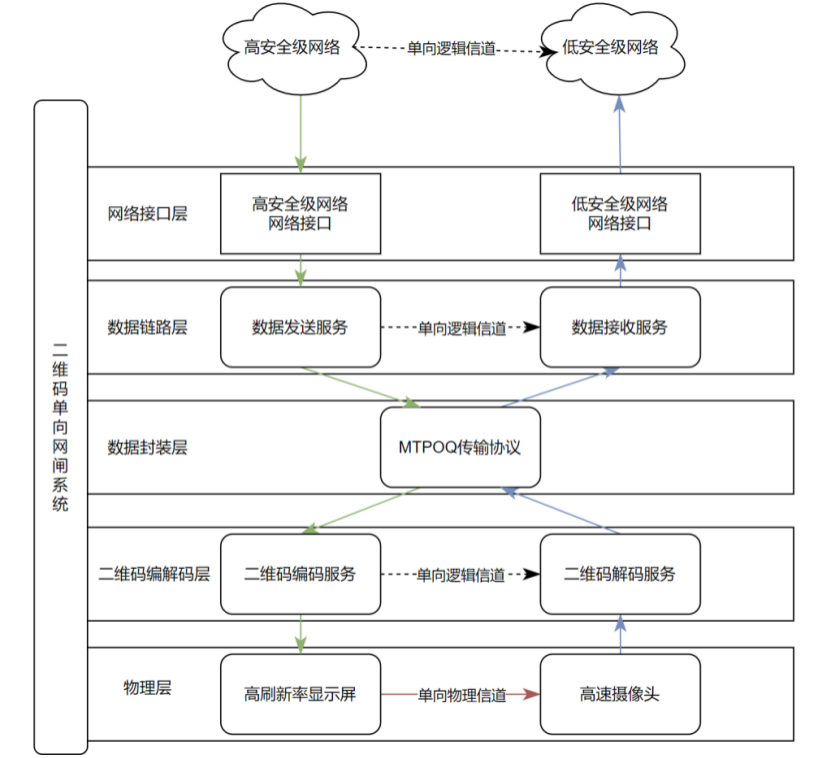
\includegraphics[scale=0.6]{figures/SStructure.png}
\caption{图像识别单向隔离装置技术架构}
\end{figure}

最底层为基于显示器与摄像头的物理单向信道。在高安全级的网络端放置一个网络数据包编码器和一个屏幕,在低安全级的网络端放置一个摄像头和一个网络数据包解码器。如此一来,由于网络包信息可以被编码为二维码展示在屏幕上而被摄像头捕获到,高安全级数据可以流向低安全级网络;由于摄像头不可能向屏幕传播任何信息,则低安全级网络中的数据不能流向高安全级网络。

二维码编解码层包括二维码编码服务与二维码解码服务。编码服务提供了高效、准确的将数据编码成为二维码能力,解码服务提供了二维码解码服务。编码服务与解码服务共同构成了二维码传输信道的数据传输实现。

数据封装层所提供的MTPOQ数据报构成了二维码的内容,也是数据抽象的重要形式无论所传输的数据是什么,协议栈都会将其作为二进制流对待。通过封装成为MTPOQ数据报可以实现数据的透明传输,其本身所携带的额外信息为上层实现检错提供了可能。

数据链路层包括数据发送服务与数据接收服务。数据发送服务将接受自上层的任务序列进行分包、封装成帧后交由下层传输,数据接收服务将下层交付的数据报进行校验、组装后提交到上层。基于MTPOQ与二维码,在数据链路层可以实现数据的无差错传输。

网络接口层提供由一般网络使用的TCP/IP协议到内部传输协议的相互转换,以免去通过本系统进行数据传输的外部开销。

针对实现基于二维码图像识别的单向隔离装置这一目标,需要一系列模块提供服务支持由普通网络数据到模块内部专有数据,再转换到普通网络数据的这一过程,以实现数据在二维码图像识别单向隔离装置上的传输。本系统是完整的单向传输系统,主要特色为基于光学的单向数据传输。系统组成模块如图4.2所示。

\begin{figure}[!htbp]
\centering
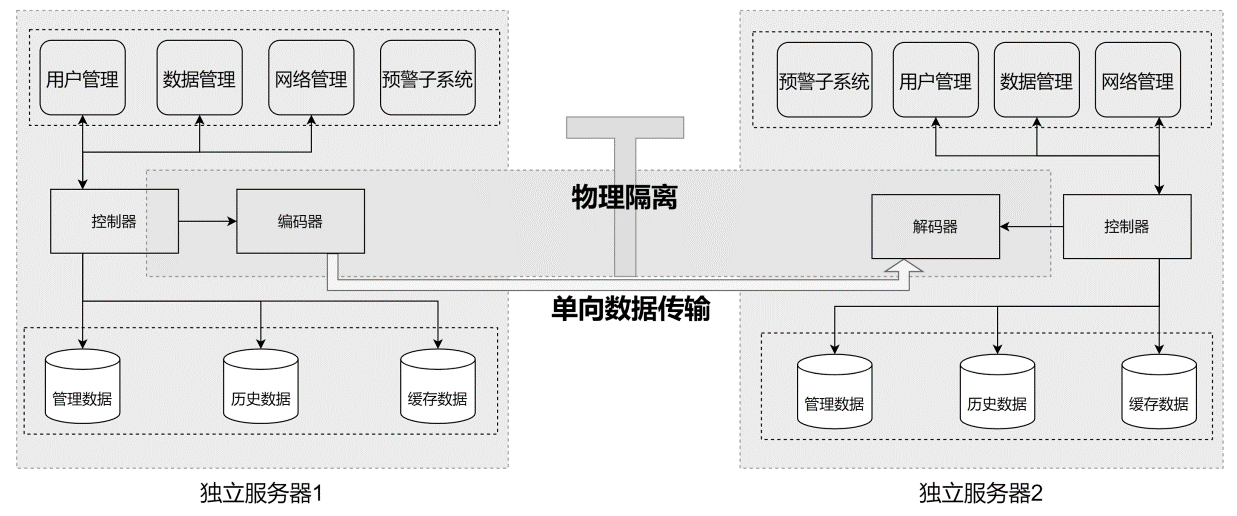
\includegraphics[scale=1]{figures/SModule.png}
\caption{系统组成模块}
\end{figure}

本系统基于二维码进行图像识别,实现数据到图像再到数据的转换。二维码的编解码速度、质量对整个系统的传输带宽至关重要。系统工作原理的大体流程如图4.3所示。

\begin{figure}[!htbp]
\centering
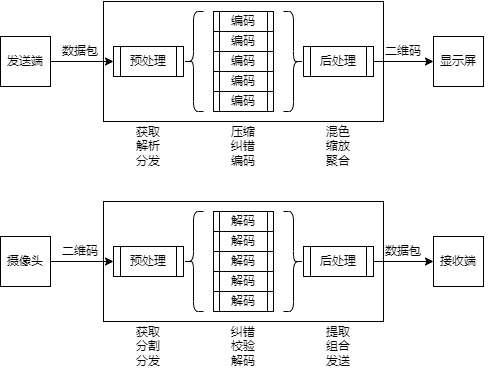
\includegraphics[scale=1]{figures/SMapReduse.png}
\caption{系统组成模块}
\end{figure}

在发送端:
\begin{itemize}
\item 编码端从上位机截获网络封包,解析应用数据;
\item 处理单元对数据进行压缩编码,然后进行纠错编码,得到图像信道数据;
\item 基于最终数据构造矩阵,形成二维编码图像;
\item 在图像信道(显示屏)上显示。
\end{itemize}

在接收端:
\begin{itemize}
\item 通过摄像机拍摄到图像,定位并分割获取图形;
\item 处理单元将图形转化为像素矩阵,识别格式和版本信息;
\item 恢复数据和纠错码,通过纠错码进行校验和纠错,得到原始网络封包;
\item 网络封包聚合后,发向接收端的传统网络信道。
\end{itemize}

\subsection{技术架构}

通过C与C++调用摄像头的API获得拍摄图片。C语言是一种广泛使用的专业语言,拥有非常高的执行效率,适合从摄像头高速获取采集到的图像数据。

软件核心编码层使用Rust语言开发。Rust语言于2010年推出,其开发的主要目的是提高整体安全性,提供优秀的模块化、良好的并行性和性能。其语言设计逻辑和本项目追求高安全、高并发和高性能的目标相吻合。Rust语言具有一系列的优秀特点,包括:不编译有错误的代码,绝佳的执行速度,硬件级代码,垃圾回收与内存安全,低成本的抽象。

操作系统使用基于Ubuntu的安全加固的Linux自制系统。针对系统安全性的措施包括了取消所有服务器的root远程ssh登录,限制su-root的用户权限,同时ssh登录端口调整,外网ssh登录全部调整;Iptables禁止除单向网闸服务外的网络权限,防止旁路资源被利用;调整密码过期时间和复杂度;调整网络泛洪、SYN等防攻击策略参数;清理服务器无效账户如Ip、news等,调整系统关键目录权限;优化服务器连接数参数;日志管理:登录认证记录等。

ZeroMQ(简称ZMQ)是一个简单易用的传输层,是一个类似于套接字库的框架,使套接字编程更简单、更干净、更强大。ZMQ提供了一个简单的套接字API,通过后台的I/O线程进行消息路由,提供多种模式的消息传输,异步地读写消息。当一个节点被移动或掉线时,ZMQ会自动连接或重新连接。\cite{郑帅2014基于}

采用国密SM4.0加密算法进行数据加密。SM4.0是中华人民共和国政府采用的一种分组加密标准,由国家密码管理局于2012年发布。组长和密钥长度均为128比特,加密算法和密钥扩展算法采用32轮的非线性迭代结构,S-box为固定的8位输入和8位输出。国密SM4.0加密算法流程如图4.4所示。

\begin{figure}[!htbp]
\centering
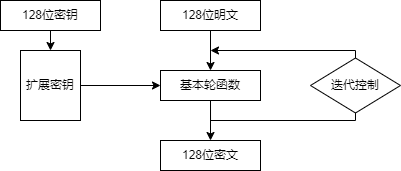
\includegraphics[scale=0.8]{figures/SM4.png}
\caption{国密SM4.0加密算法}
\end{figure}

\section{二维码编码}

二维码编码服务实现从编码队列中提取数据包,多线程地进行高速编码,并最终将编码后的二维码展示在屏幕上。

\subsection{二维码构建}

把数据包通过冗余编码方式编码为符合标准的二维码图像,在有少量遮挡和干扰的条件下要能够被识别。将标准的二维码图像融合编码为RGB三色的二维码图像。实现将编码的二维码图像编排为合理的二维码阵列,调用显示屏接口,高速展示二维码图像阵列。

为了提升IO效率,同时增加系统的带宽,在屏幕上将会展示由8个3色二维码构成的彩色二维码阵列。也就是在每次刷新的过程中将有24组二维码数据被编码为一张图片,展示在屏幕上。

由于二维码的编码过程由CPU直接执行,因此大量的高分辨率数据对程序执行是有害的。在二维码合成的过程中,通道合成与二维码拼接均在低分辨率空间下完成,直到被展示时才会被上采样为全尺寸的二维码图像。

二维码的构成与合成如图4.5所示。

\begin{figure}[!htbp]
\centering
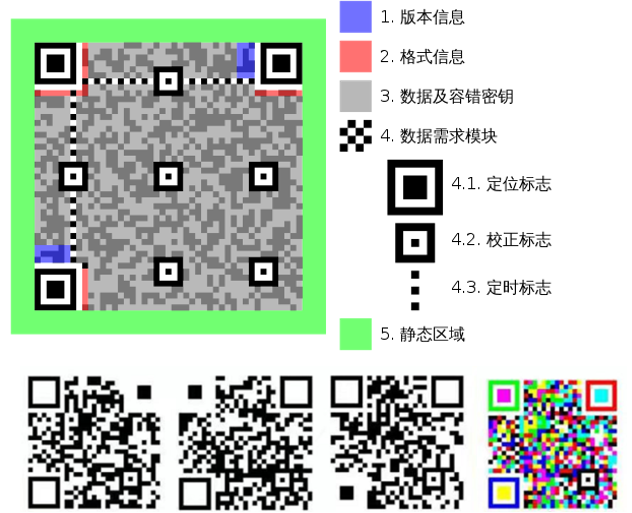
\includegraphics[scale=0.8]{figures/QR_Str.png}
\caption{二维码的构成与合成}
\end{figure}

在图像编码完成后,等待操作系统的VSYNC信号,随后通过操纵FrameBuffer将渲染完成的图像展示在屏幕上。由于显示器逐行扫描刷新的特性,需要保证显示器与系统输出的画面垂直同步以防止画面撕裂。图4.6是一个画面撕裂的例子。

\begin{figure}[!htbp]
\centering
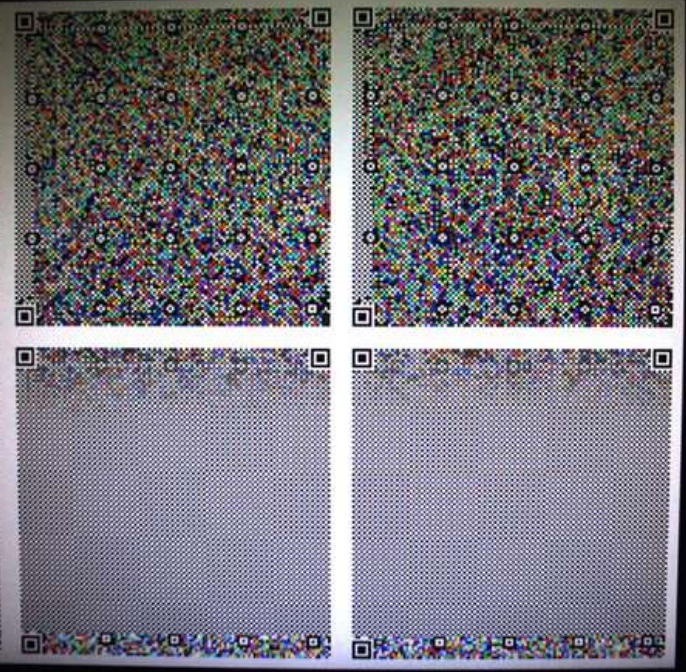
\includegraphics[scale=0.6]{figures/QR_Cap_NV.png}
\caption{发生撕裂的二维码}
\end{figure}

最终展示的效果如图4.7所示。

\begin{figure}[!htbp]
\centering
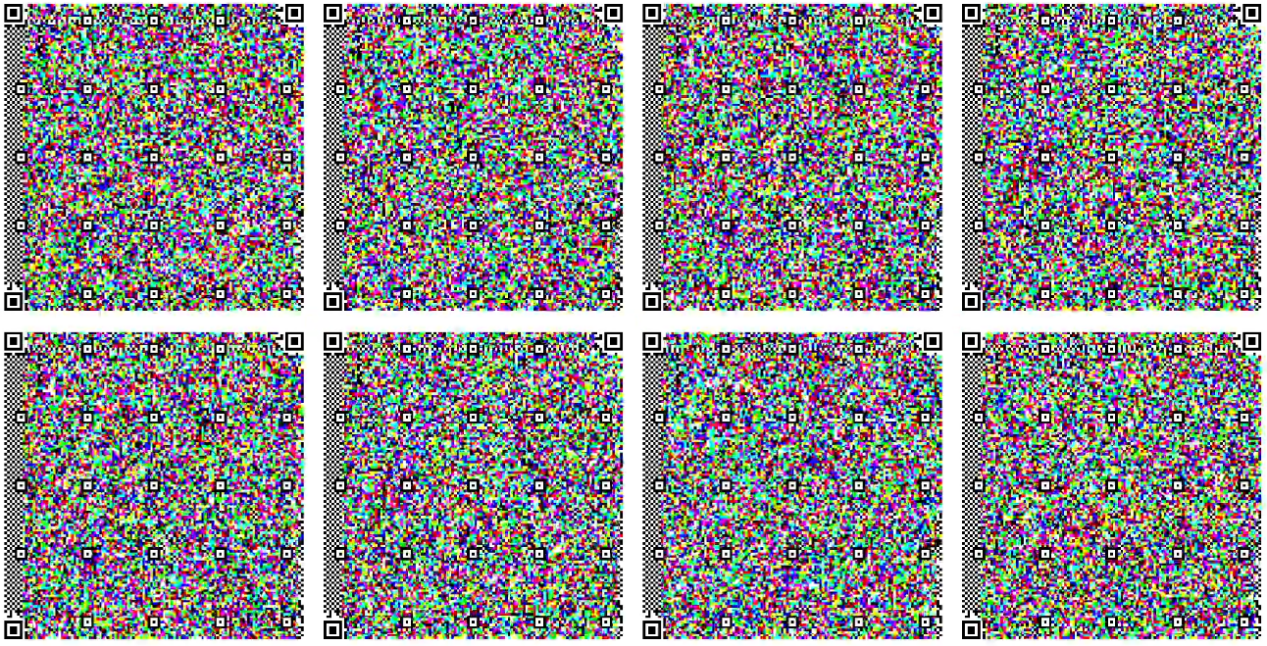
\includegraphics[scale=0.8]{figures/QR_Dp.png}
\caption{合成的彩色二维码阵列}
\end{figure}

\subsection{二维码并发编码}

为保证二维码的高速生成,需要充分利用CPU性能编码二维码,因此多线程并发不可或缺。采用线程池与队列结合的方式实现多线程并发,保证二维码的生成效率。

线程池是一组预先分配的线程,它们等待或准备处理一个任务。当程序收到一个新任务时,线程池中的随机一个线程被分配到该任务,这个线程离开线程池并处理该任务。\cite{田素贞2012基于.}然后,在该线程处理该任务时,其余的线程可以用来处理其他收到的任务。当线程处理完任务后,它返回到自由线程池中,等待新的任务并进行处理。线程池可以看做一种对于计算机资源的池化技术。具体结构如图4.8。

\begin{figure}[!htbp]
\centering
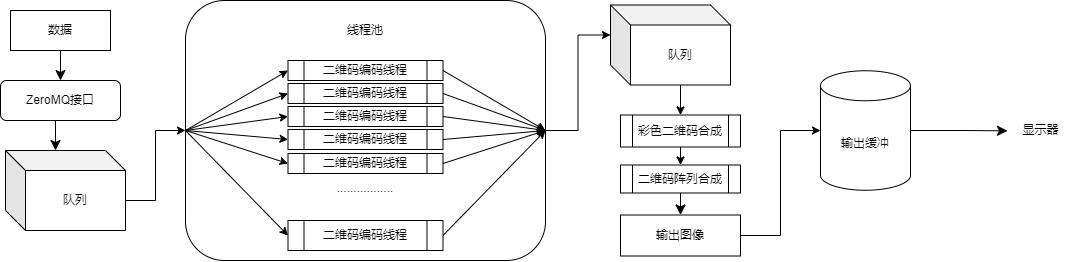
\includegraphics[scale=0.4]{figures/ENC_TP.png}
\caption{二维码线程池编码}
\end{figure}

\subsection{并发控制}

单个二维码的容量由二维码版本、纠错率与编码方式决定。受限于二维码实际用来编码数据的码元数量,单个二维码的编码容量具有上限,即不可将超过二维码容量的数据内容编码到二维码内。在发送超过单个二维码容量的数据内容时需要采取策略对数据进行分片,将超长数据编码到多个二维码中。

由于采用了线程池并发,任务的分配时机与他的完成时机不再对应,先分配的任务可能晚完成,后分配的任务也可能先完成。因此,在编入二维码的数据片段中必须有任务分段的完整位置标识。

由于图像展示逻辑只有在队列中有超过24个编码完成的二维码数据后才会被触发,因此任务片段的数量必须是24的整数倍,否则可能出现部分数据“卡死”在队列中无法被发送的情况。

\section{二维码解码}

二维码解码服务实现从二维码解码队列获取二维码,并对二维码实现精准定位,定位后分离RGB三个通道,还原为黑白通道,最后对黑白二维码进行符合协议标准的数据解码。将解码的数据包推入发射队列。

相机传感器拍摄彩色图像的方法之一是采用拜耳阵列。采用这种技术的传感器实际每个像素实际只负责感受一种指定颜色的亮度信息,需要利用反马赛克算法进行插值计算,最终获得一张彩色图像。拜耳阵列的问题之一,是在拍摄具有重复细节(即本项目中的屏幕,由于像素间存在间隙,实际存在大量重复细节)的画面时,容易产生彩色干扰信息(即摩尔纹)。而在反马赛克算法进行插值时,又会不可避免的引入色彩混叠与拉链效应,加之摄像头拍摄到的全为人工光源,实际采集到的图像与屏幕显示的图像存在较大差异。

解码服务通过摄像机API,以IPC方式,运用Request-Reply模型获得摄像机拍摄到的图片,进行解码获得二维码图片的原始数据。

对接收到的彩色二维码阵列图像,首先需要对二维码阵列进行色彩通道分离与图像区域裁切,将原始合并的(色彩通道数*阵列二维码个数)个二维码分离出来,而后逐个分别进行二维码的解码。解码测同样采用多线程并发以提高二维码解码的效率。

\subsection{二维码分割}

由摄像头拍摄到的彩色二维码阵列进行裁切,得到多个单独的二维码。在展示图片的过程中,各个二维码之间放置红色定位块来辅助进行二维码的分割。当有数据进行传输时,不显示红色定位块,兼用作跳过识别标识。

使用区块扫描法,获取连续单色区间$[(x_1,x_2),(y_1,y_2)]$,估算中心点位置,再根据估算中心进行四向线扫描,得到突变点系列$[(x_1,y_1),(x_2,y_2),(x_3,y_3),(x_4,y_4)]$,最终得到矫正后的中心点$(x_1+x_3/3+x_2+x_4/6,y_2+y_4/3+y_1+y_3/6)$。由此可得一系列分界点,依据分界点即可裁切出二维码图形。

\subsection{二维码寻像图形与矫正图像识别}

寻像图形由三个相同的位置检测图形组合构成,分别位于整个二维码的左上角、右上角和左下角。每个位置的检测图形由三个重叠的同心方块组成,包括7x7的暗模块、5x5的亮模块和3x3的暗模块。位置识别图案的模块宽度比例为1:1:3:1:1。在二维码的其他地方遇到类似图案的概率极低,并且通过二维码的掩码图案主动避免生成,因此视野中可能的二维码符号可以被快速识别。\cite{康春颖2009基于二维码技术的电子票务系统的研究}构成图像查找模式的三个位置识别图形的识别,可以精准地确定图像中符号的位置和方向。

寻像图形如下图所示:

\begin{figure}[!htbp]
\centering
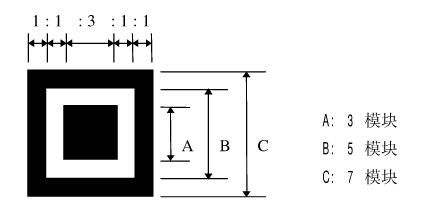
\includegraphics[scale=1]{figures/PAT_b.png}
\caption{二维码寻像图案}
\end{figure}

针对这一1:1:3:1:1的特征,使用多次穿透与模式匹配,准确获得二维码的寻像图案位置,初步推测二维码版本信息。多次穿透的方向会包括水平、垂直与主对角线方向,通过多个方向的多次穿透模板匹配,我们可以使得寻像图形中心点的绝对误差小于10\%的寻像图形长边长。基于此,我们可以准确获得二维码的寻像图案位置,初步推测二维码版本信息。
基于寻像图形的位置,我们可以指定一个范围进行模式匹配以寻找梯度校正符。梯度校正符号如下图所示:

\begin{figure}[!htbp]
\centering

\includegraphics[scale=1]{figures/PAT_s.png}
\caption{二维码梯度校正图案}
\end{figure}

由于没有计算机视觉库的支持,只能在像素空间中进行基于模板的匹配,获得校正符的位置。

\subsection{二维码并发解码}

为保证二维码的高速解码,需要充分利用CPU性能编码二维码,因此多线程并发不可或缺。采用线程池与队列结合的方式实现多线程并发,保证二维码的解码效率。

具体的实现流程与上文4.2.2节非常相似,这里不再赘述。

\section{数据发送}

在构建了二维码的编解码器后,我们即可基于二维码的编解码服务进行数据传输。本章主要内容在于说明本项目如何基于二维码进行高效率、无差错的数据传输。

在MTPOQ协议中,采用定长头部与定长尾部存放传输过程中的控制信息。原始数据作为比特流存放在数据部分中,在传输过程的任何环节都不对数据部分进行修改或访问。在编码侧,数据被分片、封装到数据报中;在解码侧,数据从数据报中被提取、组装。实现数据的透明传输。

\subsection{接收上级数据}

主线程针对物理网口,启动线程监管对于接口的连接。监管线程查询配置表,获知配置的IP、端口与协议,启动协议对应的Socket监听端口,处理到达的信息。对于UDP连接,针对到达的数据流,判断来源IP是否在白名单中,并拒绝或做接受。对于TCP连接,针对每一个TCP流,判断连接发起IP是否在白名单中,并做拒绝或启动新线程处理流。数据接收的处理流程如图4.11所示.

\begin{figure}[!htbp]
\centering
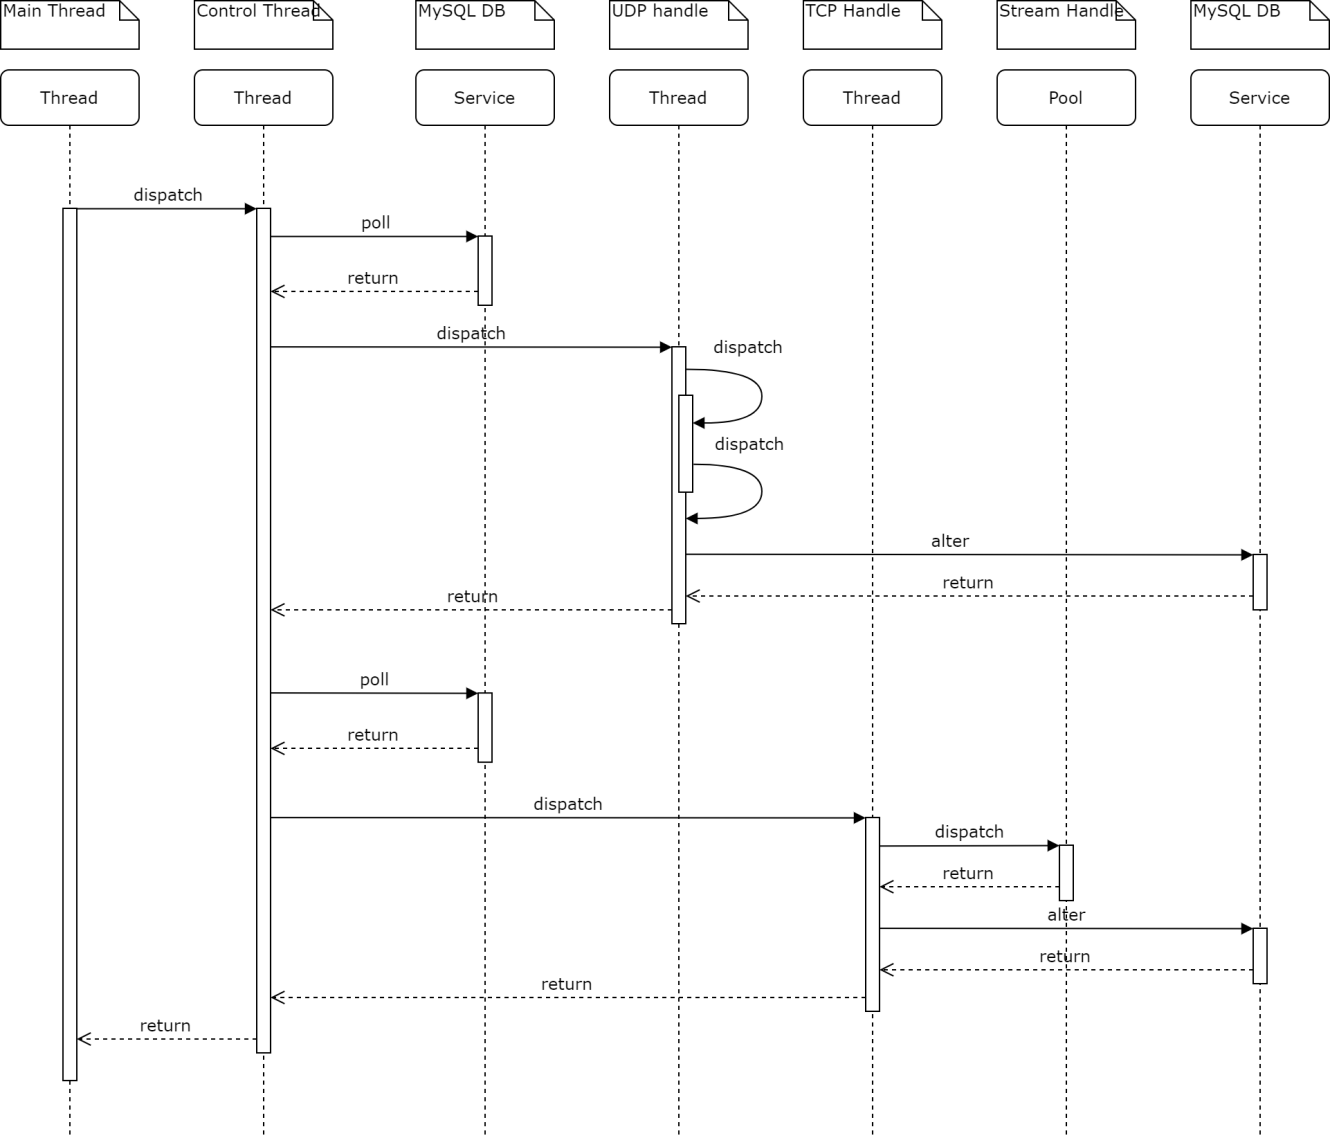
\includegraphics[scale=0.8]{figures/ST_Recv.png}
\caption{数据接收}
\end{figure}

\subsection{数据预处理}

在发送数据之前,为了传输效率考虑,我们对数据做如下的预处理:

数据流阶段。TCP是一种流协议,意味着数据以字节流的形式传递给接收者,没有"报文"或"报文边界"的概念。UDP是一个无连接协议,传输数据之前源端和终端不建立连接,当传输发生时直接将数据包发送给接收方。在数据流处理阶段,我们收集原始流式数据,获得二进制位串。

离散文件阶段。从流式数据获得的二进制位串中,解析协议内容,将数据部分缓存为文件,文件与TCP、UDP数据包内容一一对应。

文件归档阶段。TAR是Unix系统上的压缩打包工具与指令,可以将多个离散文件合并为一个归档文件,打包后的文件后缀亦为“tar”。将零散小文件组装成单个大文件,进行归档。这样做可以减少任务数量,减少大量短任务并发带来的开销。

压缩数据阶段。通过GZip对数据进行压缩编码。通过对数据进行压缩可以有效的减少文件大小,减少文件大小有两个明显的好处:一是可以减少存储空间,二是通过网络或是本项目涉及的单向网闸传输文件时,可以减少传输的时间与占用的带宽。缺点在于这将会占用编解码主机的额外算力。由于网络传输的瓶颈在于显示屏-摄像头之间传递的低效性导致的瓶颈,因此这一算力换时间的策略是值得执行的。

\subsection{数据编码}

正如同前文所提到的,单个二维码的容量有限,且我们不能保证传输信道的100\%可靠,因此,在进行MTPOQ数据的打包时,我们同时进行信源编码来提升数据的冗余度,使得最终传输的数据可以在不可靠信道上实现较高的传输成功率。在不同的MTPOQ数据包内,分散有任务的各个分片,在所有数据片段之后,我们人为的添加用于数据恢复的冗余数据片段,同样采用里德-所罗门编码,保证只要接收到足够多的正确数据就可以恢复整个任务。这一流程如图4.12所示。

\begin{figure}[!htbp]
\centering
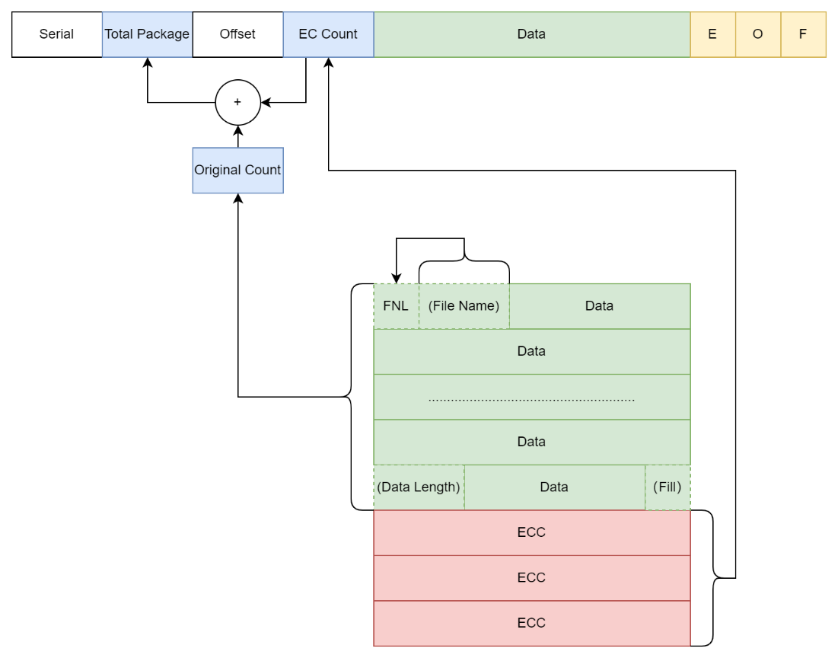
\includegraphics[scale=1.2]{figures/QR_Co.png}
\caption{数据编码}
\end{figure}

在实际传输的流程中,ECC的数量经实验,在确保99.999\%的传输可靠性的情况下,确定为:max(ceil(原始数据包数量*2 / 24) * 24, 72)。

\subsection{数据发送}

在经历前序处理流程后,将编码完成的数据通过IPC发送给二维码编码服务。数据发送服务会保证每次发送的数据包数量都向上取整到24的倍数,多余的部分由冗余度填充,以防止数据片断停留在数据管道中。流程如图4.13所示。

\begin{figure}[!htbp]
\centering
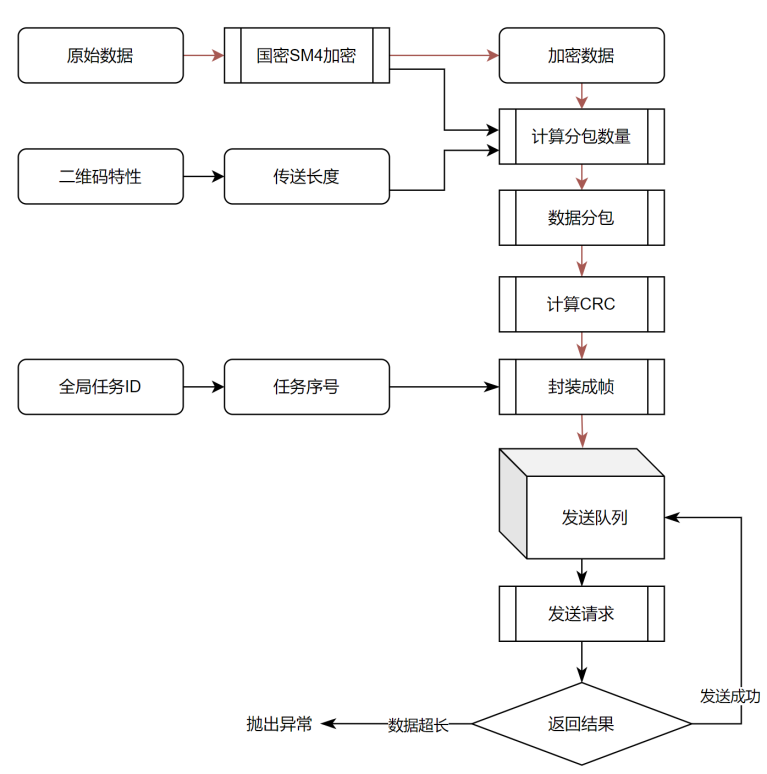
\includegraphics[scale=1.2]{figures/QR_Enc_Flow.png}
\caption{数据发送}
\end{figure}

\section{数据接收}

数据接收服务接收来自解码服务返回的MTPOQ数据报。经过数据完整性校验后,重新将分片的数据报组合为完整数据,并发送给上级组件。

\subsection{数据提取与组装}

在数据通过完整性校验而被接收后,采用[任务-分块]的二级HASH机制实现数据报片的快速、有效、离散且无冲突的临时存储。采用密码学安全的SipHash-2-4,通过让输出随机化,SipHash 能够有效减缓 Hash Flooding Attack,避免DOS的出现,保证服务的有效性。

当新任务到来时,根据序列号进行第一次HASH创建单任务数据集合,根据偏移量进行第二次HASH确定存储物理块地址,将数据报片中的数据写入内存。

任务的后续报片到来时,据序列号进行第一次HASH寻找单任务数据集合,根据偏移量进行第二次HASH确定存储物理块地址,将数据报片中的数据写入内存。

当一个任务的数据报片被全部收到时,遍历对应序列号的单任务数据集合,将离散的数据报片组装成为完整数据,之后删除任务集合中的对应序列号,释放已占用存储空间。

数据提取与组装的流程如图4.14所示。

\begin{figure}[!htbp]
\centering
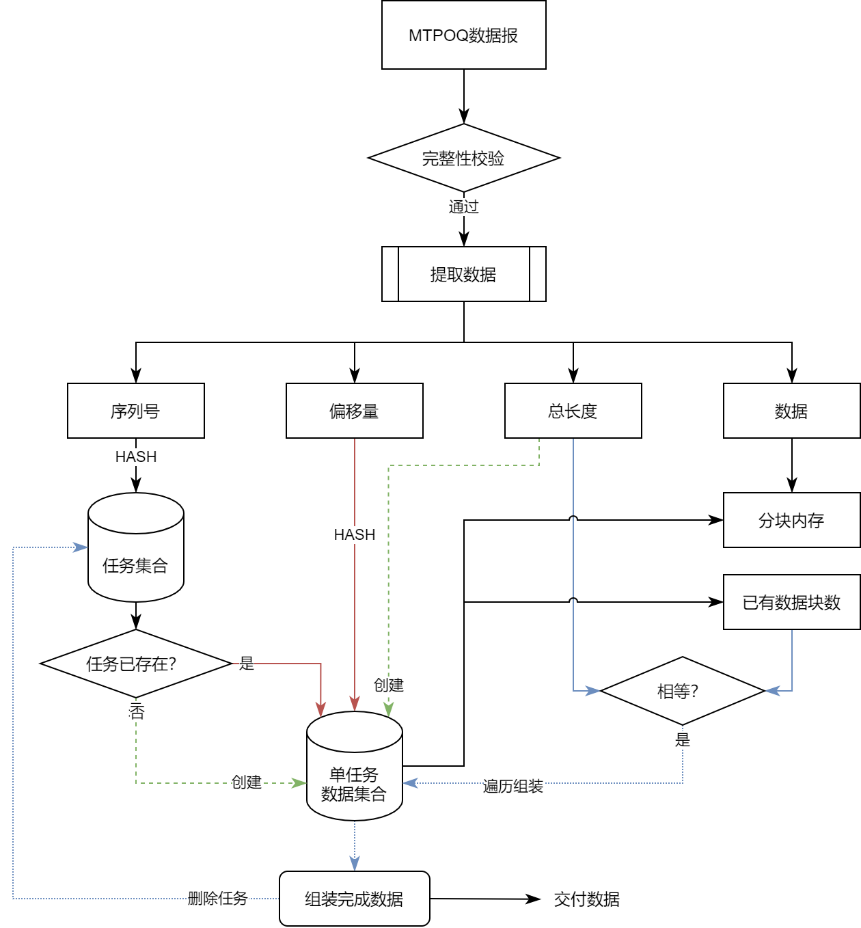
\includegraphics[scale=1]{figures/Dec_Hs.png}
\caption{数据组装流程}
\end{figure}

\subsection{数据解压缩与复原}

在发送数据时,对于一系列的TCP、UDP数据包进行了压缩打包处理以保证传输流程的高效性。在传输完成后,需要对已经压缩序列化的数据进行解包复原。此处的流程与4.4.2节为镜像关系,不再赘述。

\subsection{数据发送}

主线程接收到待发送的数据包,在数据库中查询路由表,进行协议核对,而后依照TCP与UDP分别进行处理。对UDP,直接发送到对应的目标套接字;对于TCP,尝试建立TCP连接,发送数据,然后断开TCP连接。具体流程如图4.13所示。

\begin{figure}[!htbp]
\centering
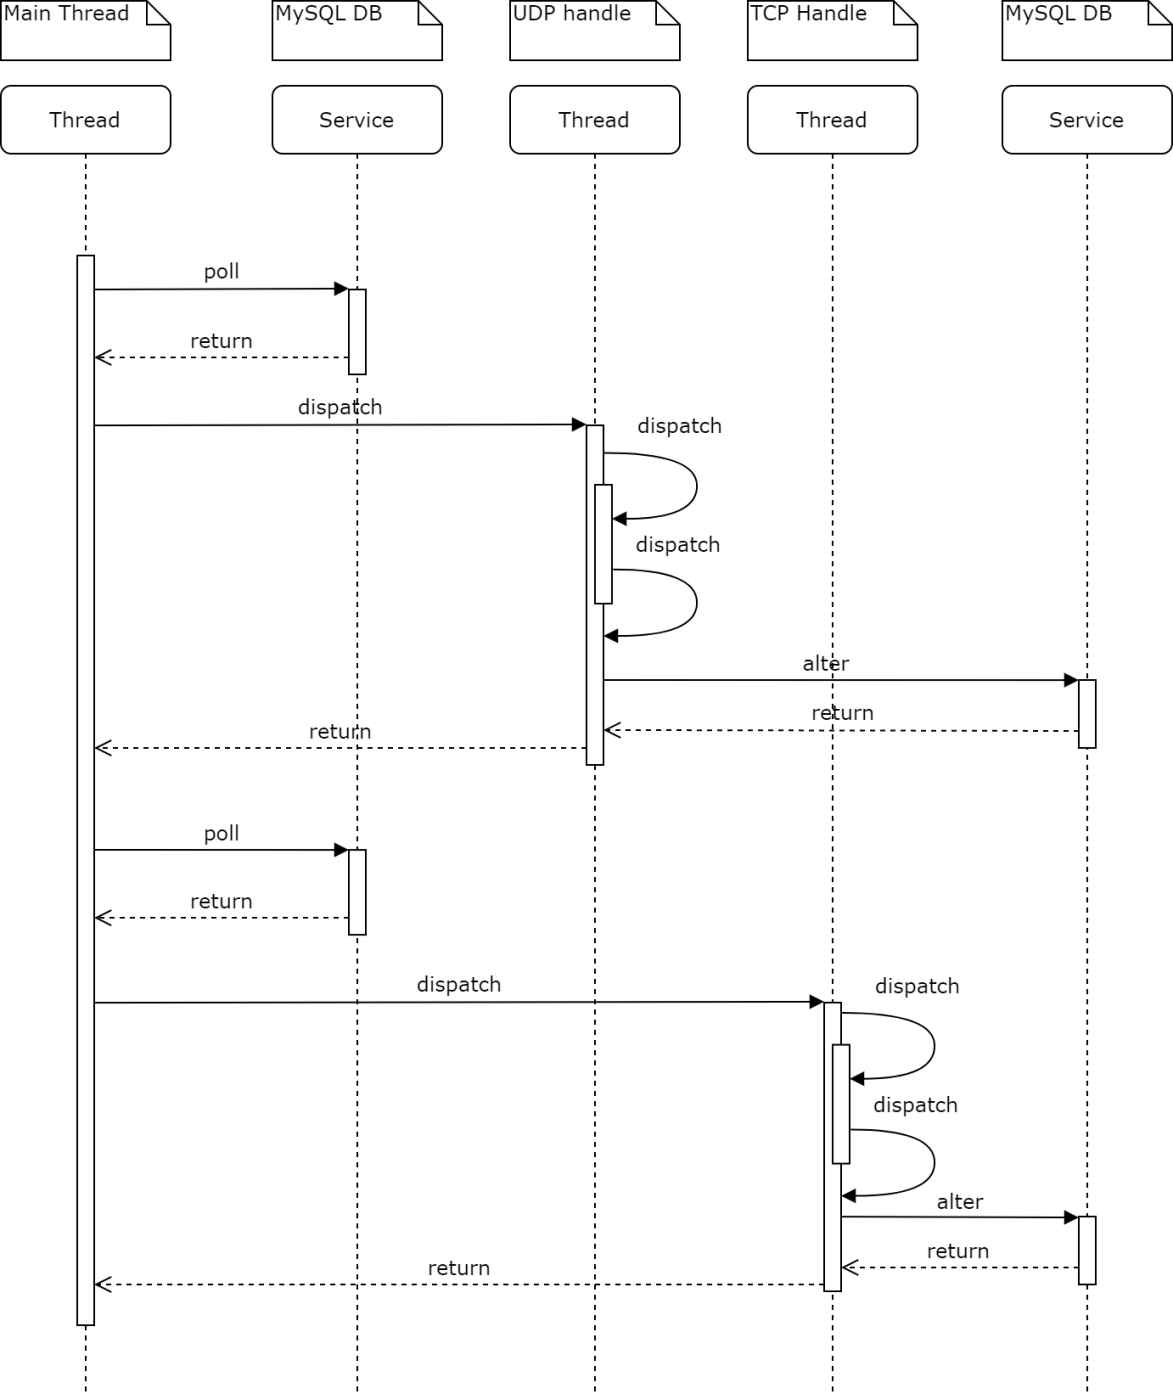
\includegraphics[scale=0.8]{figures/ST_Send.png}
\caption{数据发送}
\end{figure}

\section{数据安全性与可靠性}

对于单向网闸系统,作为网络边界管理设备,其安全性与可靠性对于整个网络系统安全可靠运行有着重大影响。针对这一问题,本项目进行了如下的实现以及优化。

\subsection{数据安全性}

实现物理隔离的通道是通过自主研发的二维码隔离通道实现的,由液晶显示器和高速摄像机组成,是本系统的核心。显示器与内部网络主机相连,高速摄像机与外部网络主机相连。内部网络主机将数据编码为二维码并显示在显示屏上。外网主通过高速摄像机机捕捉图像,进行解码,然后转发数据。物理单向隔离通道没有物理连接,确保内部和外部网络之间传输的数据的物理隔离和阻断。

采用深度定制、加固的Linux操作系统,结合内部私有协议,通过应用数据剥离、封装成图像、捕获图像、图像解码等过程,实现不同安全域之间网络数据的单向传输,从而避免系统遭受攻击与入侵。

系统将应用层的数据转换成专有的图像格式,并且对传输的数据进行安全检查,只允许安全的、可信的信息通过网闸。信息的格式、内容、时间等因素可依据用户安全策略指定。影像识别单闸对数据的交换不依赖于任何通信协议,没有建立连接会话,而是以静态的图像在内外网间传递,确保了核心应用的安全最大化。

私有的二维码协议在掩码定义、数据处理、内容分布、编码格式上与ISO国际标准二维码均不相同,内部可变参数也会更改解码的过程,外部协议无法解析私有二维码的编码内容。即使二维码图像泄露,没有协议与参数支持的情况下图像内容也无法直接解析。

\subsection{数据可靠性}

对于没有任何反馈信号、完全单向传输的物理隔绝单闸,接收端到发送端没有反向的控制帧协议,不知道对方的工作状态,不知道通信链路是否可用,无法协商双方的通信速率,发送端无法知道接收端是否准备接收数据,数据是否传输正确,不知道接收端是否正在接收数据,是否及时处理收到的数据,无法进行实时的流量控制。从理论来说,物理隔绝的单向网闸做不到绝对的可靠传输(即不重复,不遗漏,不乱序,不错误)。物理隔绝单向网闸所能做到的是尽最大可能的无差错传输,由此延长平均故障时间,提高可靠性。

二维码编码具有纠错能力。在二维码的每个数据段内散布数据与恢复内容,可以在解码同时对数据进行有限恢复,提高解码的有效性。

使用信道编码技术,利用编码方法,接收端不仅能对接收的数据进行错误检测,当检测出错误后能对错误进行定位,从而进行自动纠正。对于一个传输任务,只要接收到了足够多的正确信息,则总是可以将数据内容恢复出来\cite{杨云江2004一种在网络通信中自动纠错算法的研究}。

对传输完成的数据内容进行校验。原始的传输内嵌CRC16校验码,可以快速而有效的判别传输任务的有效性,对错误的任务进行丢弃。

\section{本章小结}

在本章,我们基于上一章所提到的二维码编解码算法,在物理硬件上实现了一条单向的、无需反向控制信息的、可以实现无差错传输的逻辑单向信道,并且有着较高的传输速率以及可靠性。由此,我们可以通过文件摆渡的方式在两个隔离的网段之间单向的传输信息。在传输文字信息的情况下,经过压缩,传输速率可以达到24Mbps,基本可以覆盖工控网络的信息流量。